% Grossmont College -- Chem 141 Lab 12: Freezing Point Depression
% Cameron Carroll
% May 2014


\documentclass[fleqn,titlepage]{article}

\renewcommand*\rmdefault{ppl}

\usepackage[version=3]{mhchem} % Package for chemical equation typesetting
\usepackage{tabu}
\usepackage{wasysym}
\usepackage{listings}
\usepackage{scrextend}
\lstset{language=Matlab}
\usepackage{multirow}

% set 1" margins on 8.5" x 11" paper
% top left is measured from 1", 1"
\topmargin 0in
\oddsidemargin 0in
\evensidemargin 0in
\headheight 0in
\headsep 0in
\topskip 0in
\textheight 9in
\textwidth 6.5in

\usepackage{graphicx} % Required for the inclusion of images

\setlength\parindent{0pt} % Removes all indentation from paragraphs

\renewcommand{\labelenumi}{\alph{enumi}.} % Make numbering in the enumerate environment by letter rather than number (e.g. section 6)

%\usepackage{times} % Uncomment to use the Times New Roman font

%----------------------------------------------------------------------------------------
% DOCUMENT INFORMATION
%----------------------------------------------------------------------------------------

\begin{document}

\begin{titlepage}
  \mbox{}\\[1.25cm]
  \textbf{\LARGE Cameron Carroll \\ Grossmont College}\\[2.25cm]
  \begin{center}
    \textbf{\huge Lab 12: \\ Molar Mass by Freezing Point Depression}\\[2.50cm]
  \end{center}
  \textbf{\LARGE Professor: Martin Larter \\ Chemistry 141-0692} \\
  \vfill
  \center{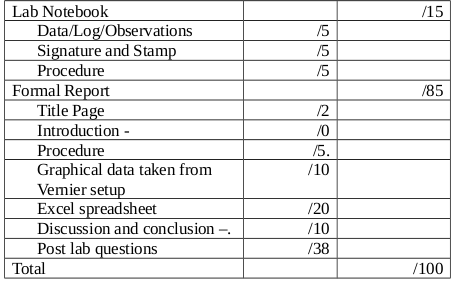
\includegraphics{./fpd_rubric}}
  \center{\textbf{\LARGE Performed --} {\LARGE May 6, 2014}}
  \center{\textbf{\LARGE Submitted --} {\LARGE May 20, 2014}}
\end{titlepage}

%----------------------------------------------------------------------------------------
% SECTION 1
%----------------------------------------------------------------------------------------
\section*{Objective}
  \paragraph{} In this experiment, we observe a colligative property: how addition of solute lowers the freezing point of a solvent. We use this depression amount to determine the molar mass of the solute.

%----------------------------------------------------------------------------------------
% SECTION 2
%----------------------------------------------------------------------------------------
\section*{Procedure}
\begin{itemize}
  \item  \textbf{Referenced From:} \\
    \begin{addmargin}[1em]{1em}
      Lehman, J. (Et al), `Determination of Molar Mass by Freezing Point Depression' \\
      Grossmont College, Chemistry 141 Lab Manual, 6th edition, pp 147-152 \\
      El Cajon, California
    \end{addmargin}
\end{itemize}

%----------------------------------------------------------------------------------------
% SECTION 3
%----------------------------------------------------------------------------------------
\newpage
\section*{Discussion \& Conclusions}
\paragraph{} I had some difficulty determining the freezing points from the graphical data: The idealized `plateau' trend was nowhere to be found -- Instead I had (mostly) continuous curves. I tried to identify the beginning and ending slope as regions where mostly temperature change and not so much phase change was taking place. Then I picked the flattest part of the center region for the first three graphs. The final graph didn't have any flat parts at all, so I selected the very center of what appeared to the the freezing region.
\paragraph{} The pure-solvent freezing points that I got were very close to the literature value of $43.2\,^{\circ}\mathrm{C}$ -- Both the points I picked were approximately $43.5\,^{\circ}\mathrm{C}$, a percent error of 0.69\%.
\paragraph{} I obtained molar masses of 111.4 and $91.18\frac{g}{mol}$ for the unknown solute. The literature value for benzoic acid is $122\frac{g}{mol}$, which gives percent errors of 8.69 and 25.3\% respectively.
\paragraph{} Upon further consideration, I want to say that the freezing point for the solution was more like $40\,^{\circ}\mathrm{C}$, which would have given a molar mass of $143.3\frac{g}{mol}$. Aside from the greater precision by deciding both graphs actually had approximately the same value, this would suggest that the unknown solute is NOT benzoic acid.


\end{document}